% 2000 年全国旧课程卷文科第 16 题：正方体内四边形投影的可能图形
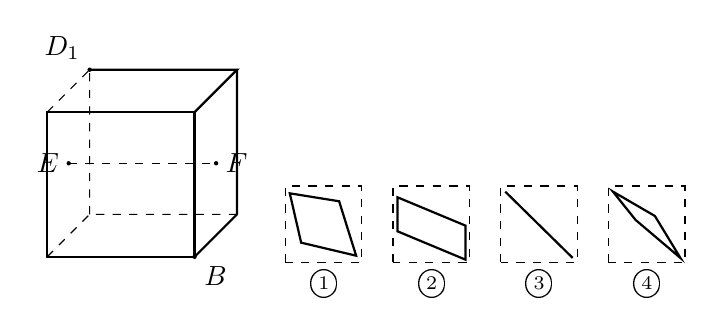
\begin{tikzpicture}[>=stealth, scale=0.72]
  \coordinate (A) at (0,0);
  \coordinate (B) at (2.6,0);
  \coordinate (C) at (3.35,0.75);
  \coordinate (D) at (0.75,0.75);
  \coordinate (A1) at (0,2.55);
  \coordinate (B1) at (2.6,2.55);
  \coordinate (C1) at (3.35,3.3);
  \coordinate (D1) at (0.75,3.3);
  \coordinate (E) at (0.38,1.65);
  \coordinate (F) at (2.98,1.65);

  \draw[thick] (A)--(B)--(B1)--(A1)--cycle;
  \draw[thick] (B1)--(C1)--(D1);
  \draw[dashed] (A)--(D)--(C) (D)--(D1) (A1)--(D1);
  \draw[thick] (B)--(C) (C)--(C1);
  \draw[dashed] (E)--(F);
  \fill (B) circle (1.1pt) node[below right] {$B$};
  \fill (D1) circle (1.1pt) node[above left] {$D_1$};
  \fill (E) circle (1.1pt) node[left] {$E$};
  \fill (F) circle (1.1pt) node[right] {$F$};

  \begin{scope}[xshift=4.2cm,yshift=-0.1cm]
    \draw[dashed] (0,0) rectangle (1.35,1.35);
    \draw[thick] (0.08,1.22)--(0.95,1.08)--(1.25,0.12)--(0.28,0.35)--cycle;
    \node[below] at (0.68,-0.08) {\textcircled{\scriptsize 1}};
  \end{scope}
  \begin{scope}[xshift=6.1cm,yshift=-0.1cm]
    \draw[dashed] (0,0) rectangle (1.35,1.35);
    \draw[thick] (0.08,1.15)--(0.08,0.55)--(1.28,0.05)--(1.28,0.65)--cycle;
    \node[below] at (0.68,-0.08) {\textcircled{\scriptsize 2}};
  \end{scope}
  \begin{scope}[xshift=8.0cm,yshift=-0.1cm]
    \draw[dashed] (0,0) rectangle (1.35,1.35);
    \draw[thick] (0.08,1.25)--(1.27,0.08);
    \node[below] at (0.68,-0.08) {\textcircled{\scriptsize 3}};
  \end{scope}
  \begin{scope}[xshift=9.9cm,yshift=-0.1cm]
    \draw[dashed] (0,0) rectangle (1.35,1.35);
    \draw[thick] (0.08,1.25)--(0.48,0.75)--(1.27,0.08)--(0.82,0.82)--cycle;
    \node[below] at (0.68,-0.08) {\textcircled{\scriptsize 4}};
  \end{scope}
\end{tikzpicture}
